\chapter{Dark Energy and Modified Gravity} % Main chapter title

\label{DE-MG} % For referencing the chapter elsewhere

%----------------------------------------------------------------------------------------


%----------------------------------------------------------------------------------------

In the introduction to this work we have motivated why an extension of General Relativity
is needed in the light of present observations and an absence of a satisfactory
solution to the cosmological constant problem.
In this chapter we will deal with the most common solution to the Dark Energy problem,
namely the addition of an extra dynamical degree of freedom in the form of a scalar field.
These models are generally called scalar-tensor (ST) \cite{Luca, Skordis, de Felice, etc.} or Modified Gravity (MG)
\cite{Silvestri, Skordis, Vernizzi, etc.} theories. 
The term scalar-tensor theories stands for theories in which a scalar field is coupled either minimally or non-minimally
to the metric tensor of gravity. On the other hand, the term 
Modified Gravity can encompass these but also other much more exotic modifications of GR, 
for example involving extra dimensions and other 
vector or tensor fields \cite{cite, bigravity, LH vector theory, dgp}. 

One can regard this extra degree of freedom as an exotic new form of matter, affecting the 
r.h.s. of the Einstein equation \ref{einstein} and generally coupled in distinct ways to different matter fields, 
or one can consider gravity to have an extra degree of freedom coupled non-minimally to the 
Ricci scalar and therefore modifying 
directly the left hand side of Einstein's field equations. The latter frame of reference
is called the Jordan frame, while the former is usually called the Einstein frame.

For theories in which all matter fields are coupled in the same way to the scalar field, both descriptions
have to be equivalent and we call them \emph{universally coupled} theories. 
For theories in which the coupling is specific to a matter field (i.e. neutrinos), the theory 
is usually formulated in the Einstein frame. These are the so-called \emph{non-universally} coupled theories.
In the following, we will use this classification to discuss the models studied in this work.

The distinction between Modified Gravity and Dark Energy is somewhat diffuse, since as mentioned above, 
an exotic form of matter in the l.h.s. of Einstein's equations can always be considered as a modification 
of the r.h.s. involving geometry. However, we will use a definition introduced recently by \cite{cite Joyce, Lombrisier, Schmidt}
which is quite practical in terms of its observable properties. 
In this definition, Dark Energy encompasses models which respect both the Weak and the Strong Equivalence
Principles and therefore do not involve extra fifth-forces that act between particles due to gravitational 
interactions. Modified Gravity encompasses models where the Strong Equivalence Principle is violated and therefore 
particles and extended bodies can have an extra "charge" that leads to the appearance of a fifth force.
As we will see below, this extra scalar degree of freedom can be thought of as being directly coupled
to the geometrical sector (the Ricci scalar in the action) or as an extra scalar field "fluid" 
coupled to matter.
If this coupling is not universal, the Weak Equivalence Principle is violated, and if, as it is 
usually the case in these models, baryons are uncoupled, these theories contain so-called 
dark sector interactions.

\begin{figure}[H]

\begin{center}
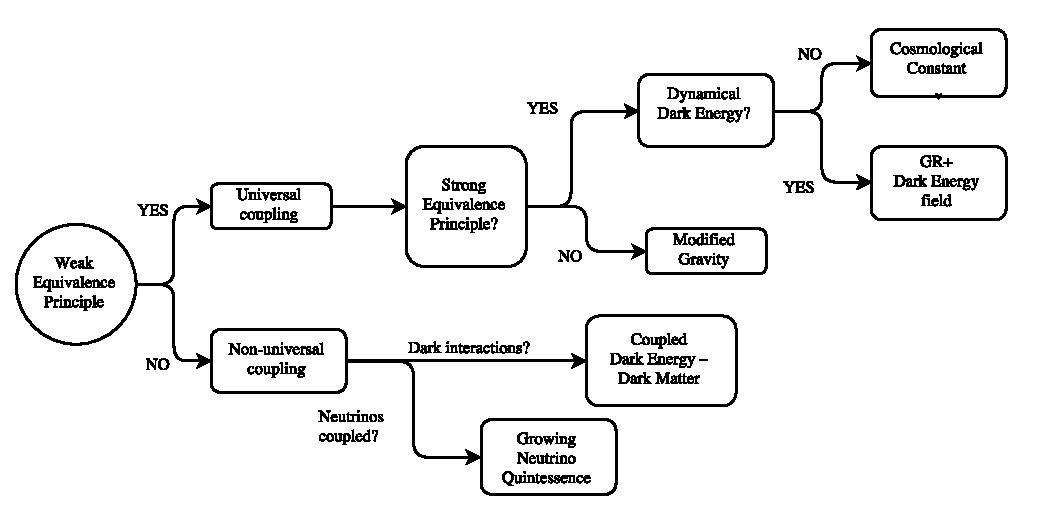
\includegraphics[width=0.99\textwidth]
{Figures/DE-MG.pdf}
\end{center}
\caption[Dark Energy - Modified Gravity Flowchart]{Distinction between Dark Energy and
Modified Gravity Theories based on the Strong and Weak Equivalence Principles (SEP and WEP), according to \cite{Joyce, Lombrisier}.
The violation of the SEP, implies the existence of an extra fifth-force among particles, 
or, equivalently, a modification of the standard Poisson equation. These are the so-called Modified Gravity theories.
If the scalar degree of freedom is not coupled to matter, then we can talk about a Dark Energy model.
In the case in which Dark Energy is not dynamical, the theory goes back to GR plus a cosmological constant.
If the WEP is violated, then not all matter species feel the same gravitational forces and therefore
there can be either dark sector interactions or neutrino--scalar-field interactions.
}
\end{figure}

In the first \cref{sec:universal-coupling} we will discuss universally coupled theories, which include ---among many others--- Quintessence, f(R),
Scalar-Tensor theories and the Horndeski theory 
(see \cite{Luca, Cliffton, Silvestri, Joyce, and more} for comprehensive reviews on Modified Gravity theories). 
We will also discuss
more general modifications of gravity which are based on the Effective Field Theory (EFT) approach to
Dark Energy and parameterizations of modifications of gravity, which
are not connected to any particular model and can accommodate any deviation from standard GR, at least at the linear 
level in perturbation theory.

In the second section, we will deal with two specific non-universally coupled models of dark energy used in this work. 
The first one is
called Coupled Dark Energy (CDE), which only couples the DE field to dark matter particles and leaves baryons uncoupled, therefore respecting solar system
constraints on gravity.
The second one, called Growing Neutrino Quintessence (GNQ), is a model in which the neutrino mass is coupled to the DE scalar field, while 
all other species remain uncoupled, which is a very phenomenologically rich theory, but possesses theoretical difficulties due to its highly non-linear evolution.
We will explain the motivations for each of these models and we will emphasize their differences in the predictions for structure formation and the background evolution of the Universe.
 
\section{The Einstein and the Jordan frames}

In this section we will review the form of the action for scalar-tensor theories in the Einstein and Jordan frames,
which are going to be useful concepts in the following chapters. For the moment we will work in units where the reduced Planck mass
$M_{Pl}^{2} = 1/(8 \pi G)$ is equal to unity.

For a scalar-tensor theory in the `Einstein-frame` the action takes the following form:
\beeqc$\label{eq:einstein-frame-action}
\mathcal{S} = \int \dx{4}{x} \sqrt{-g} \left[  \frac{1}{2} R - \frac{1}{2} g^{\mu \nu}  \partial_{\mu}\phi \partial_{\nu}\phi 
- V(\phi)    \right] - \int \dx{4}{x} \mathcal{L}_m (\tilde{g}^{(i)}_{\mu \nu} , \varPsi_m^{(i)} )
$
where generally, each matter species $\varPsi_m^{(i)}$ could be coupled to a different "effective" metric $\tilde{g}^{(i)}_{\mu \nu}$.
In the case of universal coupling (see \cref{sec:universal-coupling} below), all metrics $\tilde{g}^{(i)}$ would be identical, 
while in the case of non-universal coupling (see \cref{sec:nonuniversal-coupling} below) some of the metrics $\tilde{g}^{(i)}_{\mu \nu}$ could
be different from $g_{\mu \nu}$.
The metric $\tilde{g}^{(i)}$ is related to the metric $g$ by a conformal transformation, which takes the general form:
\beeqc$
\tilde{g}^{(i)} = \Omega^2(\phi, R) g
$
where $\Omega^2(\phi, R)$ is a function of the scalar field and in the most general case, also of the Ricci scalar, which has to be positive
to ensure attractive gravity forces.

In the Einstein frame, the gravitational part of the action looks standard, since the Ricci scalar appears alone in the action,
but the coupled matter species do not follow the geodesics given by $g$, but rather by the $\tilde g$. 
In this formulation, the energy-momentum $T^{(m)}_{\mu \nu}$ of the coupled matter species is not covariantly conserved, but rather
the sum of the energy momentum tensor of matter and the scalar field $T^{(m+\phi)}_{\mu \nu}$ is.
In the case of non-universal coupling, we will see two examples of theories formulated in the Einstein frame in \cref{sub:CDE} and \cref{sub:GNQ}.

If we have universal coupling, the action \cref{eq:einstein-frame-action} can be formulated in the "Jordan frame":
\beeqc$\label{eq:jordan-frame-action}
\mathcal{S} = \int \dx{4}{x} \sqrt{-\tilde{g}} \left[  \frac{1}{2} F(\varphi, R) - \frac{1}{2} K(\varphi) \tilde{g}^{\mu \nu}  \partial_{\mu}\varphi \partial_{\nu}\varphi 
- U(\varphi)    \right] - \int \dx{4}{x} \mathcal{L}_m (\tilde{g}_{\mu \nu} , \varPsi_m )
$
where now all matter species couple to the metric $g$, which is the same metric appearing in the gravitational part of the action.
In this frame, the Ricci scalar is non-minimally coupled to the field $\varphi$ through a function $F(R, \varphi)$ and in general, 
which can also contain a potential term for $\varphi$ and there can be an extra function $K(\varphi)$ multiplying the kinetic term of the scalar field.
In this case, matter particles follow the standard geodesics and the energy momentum tensor of the matter species is conserved.
The conformal transformation $\Omega(\varphi,R)$ relating the two frames is defined as:
\beeqp$
\Omega^2(\varphi,R) \equiv \parder{F}{R} 
$
For conformally-invariant theories (those theories in which null-geodesics are not modified), the conformal factor
just depends on the scalar field and can be written as $\Omega^2(\varphi)=\exp(2\varphi)$. 
This can be seen by performing the transformation $g \rightarrow e^{2\varphi} g$ and 
looking that at first order in the
scalar field and the gravitational potentials (which are anyway small)
this modifies the gravitational potentials as $\Phi \rightarrow \Phi-\varphi$ and $\Psi \rightarrow \Psi+\varphi$, leaving 
the Weyl (lensing) potential $\Phi_{\rm Weyl} = (1/2)(\Psi + \Phi)$ invariant.
Therefore, in this theories, the function $F$ takes the form: $F(\varphi, R) = f(\varphi)R-2U(\varphi)$, where
$f$ and $U$ are free functions of the field.
For these theories to maintain a \emph{canonical} kinetic term in the Einstein frame, a field redefinition has to be done:
\beeq$
\phi = \int \dx{}{\varphi} \sqrt{(3/2)(f_{,\varphi}/f)^2 + K/f}
$
and the potentials $U$ and $V$ are related by $V = U/f^2$.
Furthermore, in the Einstein frame, due to the conformal transformation affecting the metric in the matter Lagrangian,
particles will be coupled to the scalar field and will in general feel an extra "fifth-force", with the coupling strength
defined by:
\beeqp$
Q(\phi) \equiv -\frac{1}{2}\frac{\partial \ln f}{\partial \phi}
$
In \cref{sub:CDE} we will see an example of a constant coupling and in \cref{sub:GNQ} we will see an example of a field-dependent coupling, 
for two very distinct non-universally coupled theories.

We have to emphasize that physical measurable quantities have to be frame-independent by definition,
since this frame transformation amounts to nothing more than a coordinate and field redefinition 
and one of the principles of the GR formalism which we are not abandoning
is diffeomorphism invariance, which ensures that 
the whole theory is invariant under general coordinate transformations.


\section{Universal coupling to matter \label{sec:universal-coupling}}

Scalar-tensor theories with universal coupling written in the Jordan frame \cref{eq:jordan-frame-action}, 
encompass many of the most widely studied dark energy and modified gravity models in the literature. 
For example, $f(R)$ theories \cite{cite, many, f(R), theories} are recovered when $F(R,\varphi) = f(R)$ and $K=0$;
Brans-Dicke theory \cite{cite Brans Dicke, and, many, others} is recovered when $F(R,\varphi) = \varphi R $ and 
$K(\varphi) = \omega_{BD}/\varphi$, where $\omega_{BD}$ is the Brans-Dicke parameter and finally "k-essence" 
\cite{cite, Luca, and, some, kessence} is the case in which $F(R,\varphi) = R$ and $K$ can be a general
function of $\varphi$ and its kinetic term $(\nabla \varphi)^2$. 

There are also other theories of modified gravity with a scalar field, that are not encompassed in the set of "scalar-tensor"
theories and that have gained a lot of attention recently. Namely, Galileons \cite{cite}, Horndeski \cite{cite} 
and Beyond-Horndeski theories \cite{cite}. These theories are universally coupled to matter, are formulated
in the Jordan frame and cannot be expressed in the Einstein frame by a conformal transformation, since they contain much more complicated
derivative interactions, for example free functions of $\Box \varphi$ (see \cite{cite Zuma, Defayyet, Sawicki, Bellini}).
Horndeski's theory is an interesting case, since it is the most general theory of 
a scalar field coupled to a metric, with second order equations of motion and free of ghost instabilities. 
This theory was first formulated by Horndeski in the 1970's \cite{Horndeski}, in a purely mathematical way and was re-discovered by \cite{Defayett}
and others only in 2011 in the context of Galileons, whose simplest form (cubic Galileons) have a Lagrangian of the form:
$\mathcal{L} \propto R/2 - (\partial \varphi)^2 - (1/\Lambda_3)\Box \varphi (\partial \varphi)^2$, 
where $ \Lambda_3 $ is a free scale that can be set in the theory. They are called Galileons, 
because the equations are invariant under a general Galiliean transformation of the field $\varphi \rightarrow \varphi + b_\mu x^\mu +c$.
Beyond-Horndeski theories are extensions of Horndeski that have higher order equations of motion, but claim to be stable and free of ghosts,
\cite{cite Langlois, Gleyzes, Zuma}.

For the purposes of this work, we will now detail one of the oldest models of Dark Energy, namely
the Quintessence model \cite{Ratra-Peebles; Christof} and its extension
Coupled Quintessence introduced by \cite{Amendola_2000}.

Later on we will deal with general modifications of gravity, whose
effect on structure formation can be parameterized by two functions of
scale and time and finally we will shortly explain one of the most general approaches
to construct theories of modified gravity; the so-called Effective Field Theory of Dark Energy (EFToDE).

\subsection{Quintessence}

The Quintessence model, which takes its name from the Latin word for "fifth element"
is one of the oldest models of Dark Energy. It was introduced by several authors almost 30 years
ago \cite{Wetterich_1988, Ratra, references in Lucas, book}, motivated by studying the 
breaking of scale invariance, which could give rise to a dynamical cosmological constant.
Its Lagrangian is of the form \cref{eq:jordan-frame-action}, with
$F(\varphi, R) = R$, $K = 1$ and a potential $U(\varphi)$.
Since this is a homogeneous field without couplings, we can find its energy density and its pressure 
straightforwardly from the energy-momentum tensor of a perfect fluid in a FLRW background:
\begin{align}
&\rho_{\varphi} = -T^{0 (\varphi)}_0 = \frac{1}{2}\dot\varphi^2 + U(\varphi) \quad 
&p_{\varphi} = \frac{1}{3} T^{i (\varphi)}_i = \frac{1}{2}\dot\varphi^2 - U(\varphi) \quad ,
\end{align}
which yields the equation of state (cf. \cref{eq.1stchap}) as
\beeqp$
w_\varphi  = \frac{p_{\varphi}}\rho_{\varphi} = \frac{\dot\varphi^2 - U(\varphi)}{\dot\varphi^2 + U(\varphi)}
$
We can see that for obtaining the required behavior of $w\approx -1$ at late times, to fit 
the observations of the expansion of the Universe, we need that the kinetic term $\dot\varphi^2$
is much smaller than the potential term $U$.
From the continuity equation for a perfect fluid or from the variation of the action with respect to $\varphi$,
we can find the Klein-Gordon equation for this field:
\beeqp$
\label{eq:Klein-Gordon-Quintessence}
\ddot \varphi + 3 H \dot \varphi + U_{,\varphi} = 0
$
The dynamics and the phenomenology of this model are entirely determined by the shape of the potential
and for this there are many possibilities (see \cite[chap. 7]{amendola_dark_2010}, for a comprehensive review).
The most interesting solutions, which can alleviate the cosmological coincidence problem, are those in which the field
tracks the evolution of matter at early times ($w_\varphi \approx 1$) and then 
evolves towards an attractor (effectively independent of initial conditions) 
at late times which yields cosmic acceleration with $w_\varphi \approx -1+\xi$,
where $\xi$ is a combination of parameters from the potential and allows
to distinguish Quintessence from a simple cosmological constant at present time.
The most studied potentials are the exponential potential $U(\varphi) = U_0\exp(-\lambda \varphi)$ 
(see \cite{copeland}), where $\lambda$ is a free parameter
and the inverse power-law potential $U(\varphi) = M^{4+n} \varphi^{-n}$,
where $M$ is a mass scale of the theory.

Due to the so low energy density of dark energy ($\rho_{DE} \approx 10 ^{-120} M_{Pl}$)
compared to typical energies appearing in particle physics, it is not so easy to construct a 
viable model of Quintessence which is motivated by a fundamental theory. Nevertheless, there are 
some succesful approaches like fermion condensates, Pseudo-Nambu-Goldstone models and 
dilatonic quintessence (see \cite{amendola_dark_2010} and references therein).
These models have to satisfy that at present times dark energy is the dominating 
energy density in the Universe and therefore from the Friedmann equation:
\beeqc$
U(\varphi_0) \approx H_0^2 M_{Pl}^2
$
and if we take an inverse power law potential and take the field units to be at present $\varphi_0 = M_{Pl}$,
this would yield a mass scale $M$ of the order
of:
\beeqc$
M \approx H_0^{2/(4+n)} M_{Pl}^{(2+n)/(4+n)}
$
where, with $H_0 \approx 10^{-42} \mathrm{GeV} $, we get a mass scale of $M \approx 10^{-1} \mathrm{GeV}$
for $n=2$, which is a scale compatible with Standard Model particles.
Moreover, to satisfy the requirement of acceleration today, 
the slow-roll condition (analogous to the one in inflation \cite{infl}) must satisfy 
$ \frac{M_{Pl} V_{,\varphi \varphi}}{V(\varphi_0)} \lessapprox 1$.
Defining the mass of the scalar field $m_\varphi$ as the second derivative of the potential with respect to the field,
$m^2_\varphi \equiv  V_{,\varphi \varphi} $, yields a condition for the scalar field mass:
\beeqp$
m_\varphi \lessapprox H_0 \approx 10^{-33} \mathrm{eV}
$
So in order to be compatible with observations, 
the scalar field mass must be extremely small.
This causes a problem for all Quintessence models,
since this small mass is not stable under radiative corrections
and its potential can be disrupted under quantum corrections,
which would spoil the flatness of the potential at present times.


\subsection{Effective Field Theory of Dark Energy \label{sub:EFT-of-DE}}
\comm{delete unless there is any result you have on EFT}
\begin{itemize}
\item Another approach to construct a general model for dark energy based
on the allowed symmetries in the action.
\item Can be parametrized with the $\alpha$ functions.
\item Allows in a simple way to create theories beyond Horndeski and to
accomodate non-universal couplings.
\end{itemize}

\section{Non-universal coupling \label{sec:nonuniversal-coupling}}

\begin{itemize}
\item Motivate dark energy, the coincidence problem and a dark sector interaction
\item Explain why baryons should be uncoupled (Solar system constraints)
\end{itemize}

\subsection{Coupled Dark Energy \label{sub:CDE}}

The background evolution for the coupled DE scenario model is described
by the following equations, in which the subscripts $r$, $b$, $c$
and $\phi$, indicate radiation, baryons, cold dark matter (CDM) and
the dark energy scalar field, respectively:

\begin{eqnarray}
\ddot{\phi}+3H\dot{\phi}+\frac{dV}{d\phi} & = & \sqrt{\frac{2}{3}}\beta(\phi)\frac{\rho_{c}}{M_{Pl}}\,\,,\label{eq:quint-kleingordon}\\
\dot{\rho}_{c}+3H\rho_{c} & = & -\sqrt{\frac{2}{3}}\beta(\phi)\frac{\rho_{c}\dot{\phi}}{M_{Pl}}\,\,,\label{eq:cdm-back-density}\\
\dot{\rho}_{b}+3H\rho_{b} & = & 0\,\,,\\
\dot{\rho}_{r}+4H\rho_{r} & = & 0\,\,,\\
3H^{2} & = & \frac{1}{M_{Pl}^{2}}(\rho_{b}+\rho_{c}+\rho_{r}+\rho_{\phi})\,\,.
\end{eqnarray}


We express from now on the scalar field $\phi$ in units of the Planck
mass $M_{pl}\equiv1/\sqrt{8\pi G}$, and choose as potential $V(\phi)$
an exponential $V(\phi)=Ae^{-\alpha\phi}$ \citep{Lucchin_Matarrese_1984,Wetterich_1988}.
The coupling function $\beta(\phi)$ defines the strength of the interaction
between the DE fluid and CDM particles and in the present work we
will restrict our analysis to the simplified case of a constant coupling
$\beta(\phi)=\beta$, although in general it could be a field-dependent
quantity \cite{Amendola_2004,Baldi_2011a}.

The current constraints on a coupling to ordinary matter are very
tight. The ``post-Einstein'' coupling parameter $\bar{\gamma}$
that measures the local admixture of a spin-0 field to gravity is
constrained in Solar System experiments (see e.g. the PDG review \cite{Agashe:2014kda}
and also \citep{Will_2005,Bertotti_Iess_Tortora_2003}) roughly to
$|\bar{\gamma}|\le4\cdot10^{-5}$ . This parameter enters the modification
of the effective Newton constant as $G_{eff}=G_{N}(1-\bar{\gamma}/2)$;
in our notation, this is $G_{eff}=G_{N}(1+4\beta^{2}/3)$ (see below)
and therefore $\beta^{2}=-3\bar{\gamma}/8$. A coupling $\beta_{baryons}^{2}$
appears then constrained to be smaller than $10^{-5}$ roughly, and
we assume therefore that is completely negligible. As a consequence,
baryons follow the usual geodesics of a FLRW cosmology, which allows
coupled DE to pass the stringent local gravity constraints without
the need to employ any screening mechanism \citep{2015arXiv150203888H}.

Due to the exchange of energy between DE and CDM, the energy density
of the latter will no longer scale as the cosmic volume, and by assuming
the conservation of the CDM particle number one can derive the time
evolution of the CDM particle mass by integrating Eq.(\ref{eq:cdm-back-density})
between the present time ($z=0$) and any other redshift $z$:

\begin{equation}
m_{c}(z)=m_{c,0}e^{-\beta(\phi(z)-\phi(0))}\,\,.
\end{equation}


\subsection{Growing Neutrino Quintessence \label{sub:GNQ}}

Growing neutrino quintessence \cite{amendola_growing_2008,wetterich_growing_2007}
explains the end of a cosmological scaling solution (in which dark
energy scales as the dominant background) and the subsequent transition
to a dark energy dominated era by the growing mass of neutrinos, induced
by the change of the value of the cosmon field which is responsible
for dynamical dark energy. The dependence of the mass of neutrinos
on the cosmon (dark energy) field $\phi$, 
\begin{equation}
m_{\nu}=m_{\nu}(\phi)\propto\hat{m}_{\nu}e^{-\int\beta(\phi)d\phi}\,\,,\beta(\phi)=-\frac{\partial\ln m_{\nu}(\phi)}{\partial\phi}\label{eq: mass_def}
\end{equation}
involves the cosmon-neutrino coupling $\beta(\phi)$ which measures
the strength of the fifth force (additional to gravity). The constant
$\hat{m}_{\nu}$ is a free parameter of the model which determines
the size of the neutrino mass. (We take for simplicity all three neutrino
masses equal - or equivalently $m_{\nu}$ stands qualitatively for
the average over the neutrino species.) The special role of the neutrino
masses (as compared to quark and charged lepton masses) is motivated
at the particle physics level by the way in which neutrinos get masses
\cite{wetterich_growing_2007}. Growing neutrino quintessence with
a sufficiently large negative value of $\beta$ successfully relates
the present dark energy density and the mass of the neutrinos. The
evolution of the cosmon is effectively stopped once neutrinos become
non-relativistic. Dark energy becomes important now because neutrinos
become non-relativistic in a rather recent past, at typical redshifts
of about $z=5$ \cite{mota_neutrino_2008}. In this way, the ``why
now problem'' is resolved in terms of a ``cosmic trigger event''
induced by the change in the effective neutrino equation of state,
rather than by relying on the fine tuning of the scalar potential.
This differs from other mass varying neutrino cosmologies (usually
known as MaVaN's) \cite{brookfield_cosmology_2007,la_vacca_mass-varying_2013,bi_cosmological_2005,fardon_dark_2004,kaplan_neutrino_2004,spitzer_stability_2006,takahashi_speed_2006}.
Some of the observational consequences of those models were studied
in \cite{la_vacca_mass-varying_2013,kaplan_neutrino_2004} and more
recently a new scalar field - neutrino coupling that produces viable
cosmologies was proposed in \cite{simpson_dark_2016}. A viable cosmic
background evolution of growing neutrino quintessence offers interesting
prospects of a possible observation of the neutrino background.

The case in which the coupling $\beta$ is constant has been largely
investigated in literature at the linear level \cite{mota_neutrino_2008},
in semi-analytical non-linear methods \cite{wintergerst_clarifying_2010,wintergerst_very_2010,brouzakis_nonlinear_2011},
joining linear and non-linear information to test the effect of the
neutrino lumps on the cosmic microwave background \cite{pettorino_neutrino_2010}
and within N-Body simulations \cite{ayaita_neutrino_2013,ayaita_structure_2012,baldi_oscillating_2011,ayaita_nonlinear_2016}.
For the values of $\beta$ ($\beta\gtrsim10^{3}$) needed for dark
energy to dominate today, the cosmic neutrino background is clumping
very fast. Large and concentrated neutrino lumps form and induce very
substantial backreaction effects. These effects are so strong that
the deceleration of the evolution of the cosmon gets too weak, making
it difficult to obtain a realistic cosmology \cite{fuhrer_backreaction_2015}.

In this paper we instead consider the case in which the neutrino-cosmon
coupling $\beta(\phi)$ depends on the value of the cosmon field and
increases with time. In a particle physics context this has been motivated
\cite{wetterich_growing_2007} by a decrease with $\phi$ of the heavy
mass scale (B-L-violating scale) entering inversely the light neutrino
masses. In this scenario $\beta(\phi)$ has not been large in all
cosmological epochs - the present epoch corresponds to a crossover
where $\beta$ gets large. A numerical investigation \cite{baldi_oscillating_2011}
of this type of model has revealed compatibility with observations
for the case of a present neutrino mass $m_{\nu,0}=0.07$ eV. In the
present paper we investigate the dependence of cosmology on the value
of the neutrino mass by varying the parameter $\hat{m}_{\nu}$ in
eq. \ref{eq: mass_def}. For large neutrino masses we find a
qualitative behavior similar to the case of a constant neutrino-cosmon
coupling $\beta$, with difficulties to obtain a realistic cosmology.
In contrast, for small neutrino mass, the neutrino lumps form and
dissolve, with small influence on the overall cosmological evolution.
In this case, the neutrino-induced gravitational potentials are found
to be much smaller than the ones induced by dark matter. As we will
discuss in this paper, it will not be easy to find observational signals
for the neutrino lumps. In-between the regions of small and large
neutrino masses we expect a transition region for intermediate neutrino
masses where, by continuity, observable effects of the neutrino lumps
should show up.


\subsubsection{Growing neutrinos with varying coupling}

We consider here cosmologies in which neutrinos have a mass that varies
in time, along the framework of ``varying growing neutrino models''
\cite{wetterich_growing_2007}. As long as neutrinos are relativistic,
the coupling is inefficient and the dark energy scalar field $\phi$
rolls down a potential, as in an early dark energy scenario. As the
neutrino mass increases with time, neutrinos become non-relativistic,
typically at a relatively late redshift $z\approx4-6$ \cite{pettorino_neutrino_2010}.
This influences the evolution of $\phi$, which feels the effect of
neutrinos via a coupling to the neutrino mass $m_{\nu}(\phi)$. The
evolution of the scalar field slows down and practically stops, such
that the potential energy of the cosmon behaves almost as a cosmological
constant at recent times. In other words, in these models the cosmological
constant behavior observed today is related to a cosmological trigger
event (i.e. neutrinos becoming non-relativistic) and the present dark
energy density is directly connected to the value of the neutrino
mass. In the following we will detail the formalism and equations
used to describe the cosmological evolution of the model.

We start with the linearized Friedman-Lemaitre-Robertson-Walker metric
in the Newtonian gauge: 
\begin{equation}
ds^{2}=-(1+2\Psi)dt^{2}+a^{2}(1-2\Phi)d\mathbf{x}^{2}\,\,.
\end{equation}
Moreover, we use a quasi-static approximation for sub-horizon scales
($H/k\ll1$) which allows us to neglect time derivatives with respect
to spatial ones. Then the quasi-static, first-order perturbed Einstein
equations, are the Poisson equation \cite{ma_cosmological_1994}

\begin{equation}
k^{2}\Phi=4\pi Ga^{2}\delta T_{0}^{0}\,\,,\label{eq:Poisson}
\end{equation}
and the ``stress'' equation 
\begin{equation}
k^{2}(\Phi-\Psi)=12Ga^{2}(\bar{\rho}+\bar{P})\sigma\,\,,\label{eq:stress-phipsi}
\end{equation}
where $\delta T_{0}^{0}$ is the perturbation of the $0-0$ component
of the energy momentum tensor $T_{\mu\nu}$ and $\sigma$ is the anisotropic
stress of the fluid which depends on the traceless component of the
spatial part of the energy-momentum tensor, $T_{j}^{i}-\delta_{j}^{i}T_{k}^{k}/3$.
This stress tensor is in our case only important for relativistic
particles (i.e. the neutrinos). The source term of the Poisson equation
\ref{eq:Poisson} will contain contributions from all matter
species (dark matter \& neutrinos) and from the cosmon field. It is
proportional to the total density contrast $\delta\rho_{t}=\delta\rho_{\nu}+\delta\rho_{m}+\delta\rho_{\phi}$.

The cosmon field can be described through a Lagrangian in the standard
way 
\begin{equation}
-\mathcal{L_{\phi}}=\frac{1}{2}\partial^{\nu}\phi\partial_{\nu}\phi+V(\phi)
\end{equation}
where for this work we choose an exponential potential $V(\phi)\propto e^{-\alpha\phi}$.
The field dependent mass (eq.\ref{eq: mass_def}) allows for
an energy-momentum transfer between neutrinos and the cosmon, which
is proportional to the trace of the energy momentum tensor of neutrinos
$T_{(\nu)}$ and to a coupling parameter $\beta(\phi)$ 
\begin{align}
\nabla_{\eta}T_{(\phi)}^{\mu\eta}= & +\beta(\phi)T_{(\nu)}\partial^{\mu}\phi\,\,\,,\label{eq:continuity-phi}\\
\nabla_{\eta}T_{(\nu)}^{\mu\eta}= & -\beta(\phi)T_{(\nu)}\partial^{\mu}\phi\,\,\,.\label{eq:continuity-nu}
\end{align}


The cosmon is the mediator of a fifth force between neutrinos, acting
at cosmological scales. Its evolution is described by the Klein-Gordon
equation sourced by the trace of the energy-momentum tensor $T_{(\nu)}$
of the neutrinos,

\begin{equation}
\nabla_{\mu}\nabla^{\mu}\phi-V'(\phi)=\beta(\phi)T_{(\nu)}.\label{eq:klein-gordon-equation}
\end{equation}
As long as the neutrinos are relativistic ($T_{(\nu)}=0)$ the source
on the right hand side vanishes. During this time, the coupling has
no effect on the evolution of $\phi$. While the potential term $\sim V'$
drives $\phi$ towards larger values, the term $\sim\beta$ has the
opposite sign and stops the evolution effectively once $\beta T_{(\nu)}$
equals $V'$. The trace of the energy momentum tensor $T_{\nu}$,
entering eq.\ref{eq:klein-gordon-equation} is equal to: 
\begin{equation}
T_{\nu}=m_{\nu}(\phi)\tilde{n}(\phi)\label{eq:trace}
\end{equation}
where $\tilde{n}_{\nu}(\phi)=n_{\nu}(\phi)/\gamma$ is the ratio of
the number density of neutrinos $n_{\nu}$, divided by the relativistic
$\gamma$ factor. Eq.\ref{eq:trace} is valid for both relativistic
and non-relativistic neutrinos. Here we consider a coupling $\beta$
between neutrino particles and the quintessence scalar field $\phi$
as a field dependent quantity: 
\begin{equation}
\beta(\phi)\equiv-\frac{1}{\phi_{c}-\phi}\,.\label{eq:beta-of-phi}
\end{equation}
From eq.\ref{eq: mass_def} the neutrino mass is then given
by: 
\begin{equation}
m_{\nu}(\phi)=\frac{\bar{m}_{\nu}}{\phi_{c}-\phi}\,.\label{eq:mnu-of-phi}
\end{equation}
Here $\phi_{c}$ denotes the asymptotic value of $\phi$ for which
$\beta$ and $m_{\nu}(\phi)$ would formally become infinite. By an
additive shift in $\phi$ it can be set to an arbitrary value, e.g.
$\phi_{c}=0$. We consider the range $\phi<\phi_{c}$. The divergence
of $\beta$ for $\phi\rightarrow\phi_{c}$ in eq.\ref{eq:beta-of-phi}
is not crucial for the results of the present paper - $\beta$ and
$m_{\nu}$ never increase to large values, such that the immediate
vicinity of $\phi_{c}$ plays no role.

The coupling induces a total force acting on neutrinos given by $\nabla(\Phi_{\nu}+\beta\delta\phi)$
and appearing in the corresponding Euler equation \cite{pettorino_neutrino_2010},
as usual in coupled cosmologies \cite{baldi_hydrodynamical_2010}.
For values $2\beta^{2}>1$ the fifth force induced on neutrinos by
the cosmon becomes larger than the gravitational attraction. For the
large values of $|\beta|\approx10^{2}$ reached during the cosmological
evolution, the attraction induced by the cosmon gives rise to the
formation of neutrino lumps. As shown in \cite{mota_neutrino_2008,pettorino_neutrino_2010}
this represents the major difficulty encountered within growing neutrino
models and also, simultaneously, one of its clearest predictions with
respect to alternative dark energy models: the presence of neutrino
lumps at scales of $\approx10$ Mpc or even larger, depending on the
details of the model \cite{mota_neutrino_2008}. Since the attractive
force between neutrinos is $10^{4}$ times bigger than gravity, therefore
also the dynamical time scale of the clumping of neutrino inhomogeneities
is a factor $10^{4}$ faster than the gravitational time scale. Even
the tiny inhomogeneities in the cosmic neutrino background grow very
rapidly non-linear. The impact of such structures, has been shown
to depend crucially on the strength of backreaction effects \cite{ayaita_structure_2012,ayaita_nonlinear_2016}.
For constant coupling, the effect of backreaction is strong and can
lead to neutrino lumps with rapidly growing concentration, reaching
values of the gravitational potential which exceed observational constraints.
The effect is so strong that it is able to destroy the oscillatory
effect first encountered in \cite{baldi_hydrodynamical_2010}, in
which neutrino lumps were forming and then dissipating. No realistic
cosmology has been found in this case \cite{fuhrer_backreaction_2015}.
With the varying coupling of eq.\ref{eq:beta-of-phi} a similar
behavior will be found for large neutrino masses. For small neutrino
masses the oscillatory effects will be dominant and realistic cosmologies
seem possible \cite{ayaita_nonlinear_2016}.




%\subsection{Non-universal couplings in EFT}
%\comm{delete this paragraph}
%Paper by Gleyzes
%\section{Non-local gravity}
%\begin{itemize}
%\item Non-local terms in the action, like inverses of the box operator acting
%on the Ricci scalar, are motivated by quantum gravity corrections
%\item Non-local expressions can be localized in terms of scalar fields.
%\item There are the same number of parameters as in LCDM, instead of $\Lambda$
%there is a mass parameter.
%\item Seems to give a very good fit to present observations.
%\end{itemize}